\section{Processi Stocastici}
    I \emph{processi stocastici} sono segnali continui ma aleatori: é un set di variabili aleatorie indicizzate nel tempo.
    \paragraph{Propietá:}
        \begin{itemize}
            \item {Sono funzione del tempo.}
            \item {Sono funzioni aleatorie, non possiamo predire, prima di condurre l'esperimento, l'andamento del segnale ma 
            possiamo analizzarne un andamento probabilistico tramite degli indici come: potenza media, funzioni di correlazione e spettro dell'energia}
        \end{itemize} 
        \begin{figure}[H]
            \centering
            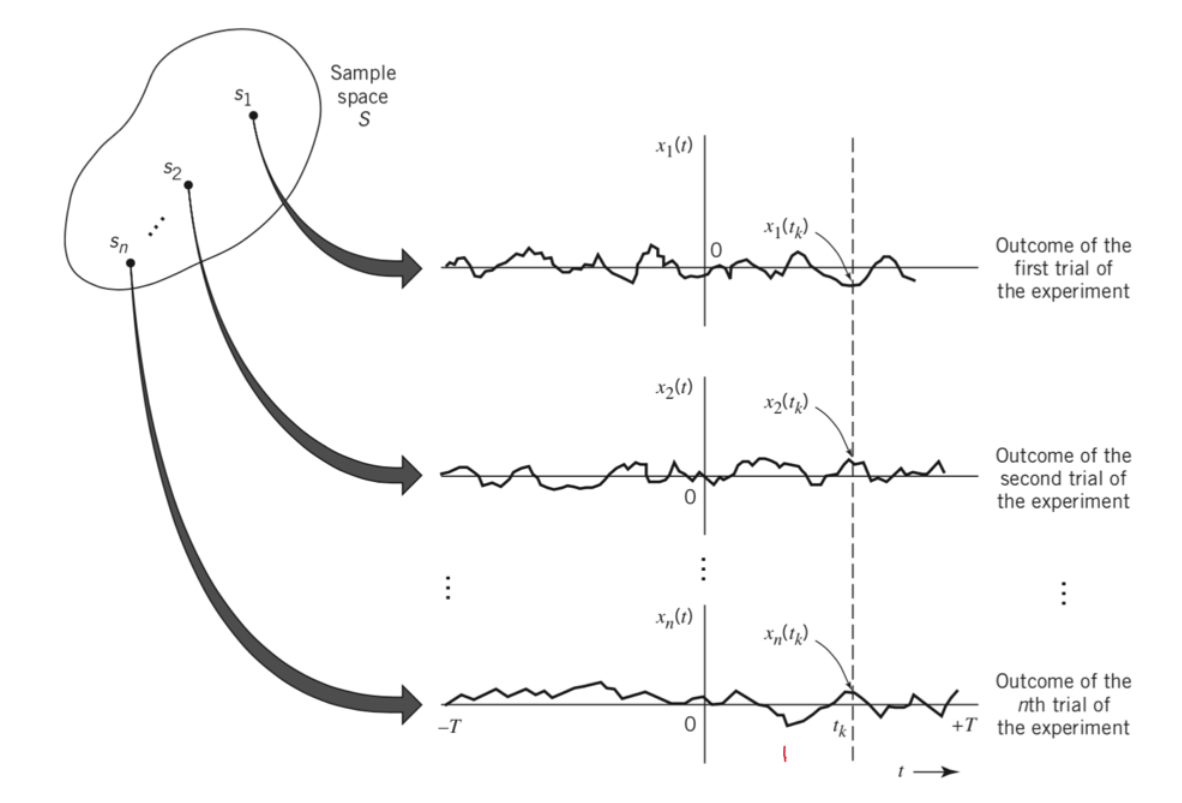
\includegraphics[width = 6cm]{media/processi stocastici.png}
        \end{figure}
        al campionamento $t_k$ ho un set di variabili aleatorie. L'aletorietá puó essere derivante da uno o piú fattori,
        ad esempio in una funzione cosinusoidale $Acos(2\pi f_ct+\Theta)$ possono essere aleatorie ampiezza, frequenza e fase.

    \subsection{Valore medio}
        Consideriamo un processo stocastico reale $X_{(t)}$, il valore medio é l'expectation della variabile aleatoria ottenuta campionando
        il processo al tempo $t$:
            \[
                \mu_{X(t)} = \mathbb{E}[X_{(t)}] = \int_{-\infty}^{\infty}xf_{X_{(t)}(t)}dt
            \]
        ad ogni istante di tempo $t$ ho una nuova variabile aleatoria per questo é funzione del tempo.
    \subsection{Autocorrelazione}
        Consideriamo un processo stocastico reale $X_{(t)}$ e due variabili aleatorie associate $X_{(t_1)}$ e $X_{(t_2)}$. 
        L'autocorrelazione é l'expectation del prodotto delle due variabili aleatorie:
        \[
            R_{XX(t_1,t_2)} = \mathbb{E}[X_{t_1}X_{t_2}] = \int_{-\infty}^{\infty}\int_{-\infty}^{\infty} x_1x_2f_{X_{(t_1)},X_{(t_2)}(x_1,x_2)}dx_1dx_2
        \]
        \subsubsection{Propietá della autocorrelazione $R_x$}
            \begin{itemize}
                \item {Paritá: $R_{X(\tau)} = R_{X(-\tau)}$}
                \item {$R_{X(0)}\geq \underset{Val.\ Massimo}{\underbrace{\left|R_{X(\tau)}\right|}}$: Cosa rappresenta?
                    \begin{align}
                        R_{X(\tau)} &= \mathbb{E}[X_{(t_1)}X_{(t_2)}]=\eval*{\mathbb{E}[X_{(t)}X_{(t-\tau)}] }_{\tau = 0} \nonumber \\
                        R_{X(0)}    &= \underset{Potenza}{\underbrace{\mathbb{E}[|X|^2]}} = \int_{-\infty}^{\infty} x^2f_{X_{(t)}(t)}dx \nonumber
                    \end{align}
                    coincide con la potenza del processo SSL.
                }
            \end{itemize}
        \subsubsection{Sigificato fisico dell'autocorrelazione}
            La funzione di autocorrelazione ci fornisce la possibilitá di descrivere l'indipendenza di due variabili aleatorie ottenute dal campionamento
            del processo stocastico $X_{(t)}$ a tempi divesti. Piú il processo stocastico $X_{(t)}$ cambia nel tempo, piú rapidamente la funzione di autocorrelazione 
            scenderá dal suo massimo $R_{XX(0)}$
            \begin{figure}[H]
                \centering
                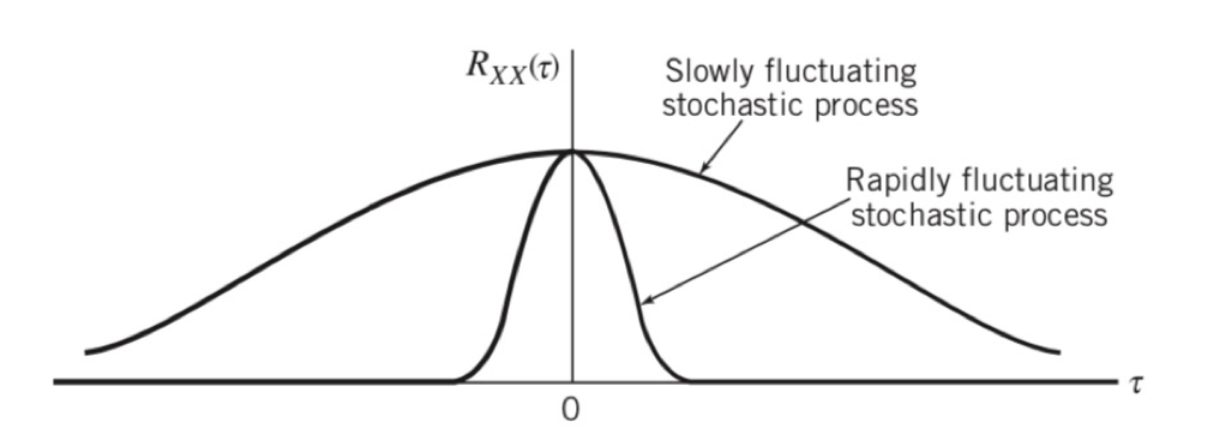
\includegraphics[width = 8cm]{media/autocorrelazione stocastica.png}
            \end{figure}
    \subsection{Sitemi Stazionari in Senso Lato (SSL)}\label{Sitemi Stazionari in Senso Lato (SSL)}
        Un processo stocastico $X_{(t)}$ si dice Stazionario in Senso Lato (SSL) se:
        \begin{itemize}
            \item {Il valore medio del processo $X_{(t)}$ é costante $\forall t$:
                \[
                    \mu_{X(t)} = \mathbb{E}[X_{(t)}] \overset{SSL}{\Rightarrow} \mu_{X}    
                \]
            }
            \item {La funzione di autocorrelazione del processo $X_{(t)}$ dipende solamente dalla differenza tra la differenza 
                tra due tempi qualsiasi al quale il processo é campionato:
                \[
                    R_{XX(t_1,t_2)} = \mathbb{E}[X_{(t_1)}X_{(t_2)}] \overset{SSL}{\Rightarrow} R_{X(t_1-t_2)} = R_{X(\tau)}      
                \]
                Se il processo dipende solo da $\tau$ posso farne la $TCF$ e analizzarne la densitá spettrale. 
                }
        \end{itemize} 
        \subsubsection{Trasmissione di un SSL in un sistema LTI-Filter}
            Supponiamo di avere un processo stocastico $X_{(t)}$ in ingresso ad un sistema LTI-Filter di risposta $h_{(t)}$,
            producendo un nuvo processo stocastico $Y_{(t)}$
            \begin{figure}[H]
                \centering
                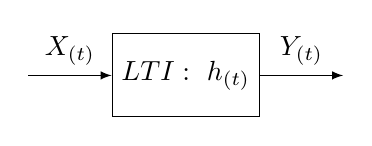
\begin{tikzpicture}[
                        node distance=2cm,
                        >=latex
                    ]
                    % Blocks
                    \node [coordinate] (input) {};
                    \node [rectangle, draw,minimum height=3em, minimum width=3em,right of=input] (filter) {$LTI:\ h_{(t)}$};
                    \node [coordinate, right of=filter] (output) {$s_{(t)}$};
                
                    % Connections
                    \draw [->] (input) --node[above]{$X_{(t)}$} (filter);
                    \draw [->] (filter) --node[above]{$Y_{(t)}$} (output);
                \end{tikzpicture}    
            \end{figure}
            l'uscita $Y_{(t)}$ si calcola con la convoluzione:
            \[
                Y_{(t)} = X_{(t)} \otimes h_{(t)} = \int_{-\infty}^{\infty} X_{(\alpha)} h_{(t-\alpha)} d\alpha
            \]
            Calcoliamone gli indici:
            \begin{itemize}
                \item {
                    Valore medio:
                    \begin{align}
                        \mu_Y &= \mathbb{E}[Y_{(t)}] =\mathbb{E}[X_{(t)} \otimes h_{(t)}] = \mathbb{E}\left[\int_{-\infty}^{\infty} X_{(\alpha)} h_{(t-\alpha)} d\alpha\right]\nonumber \\
                              &\overset{\ref{linearita expectation}}{=} \int_{-\infty}^{\infty} \mathbb{E}[X_{(\alpha)}] h_{(t-\alpha)} d\alpha = \int_{-\infty}^{\infty} \mu_{X_{(\alpha)}} h_{(t-\alpha)} d\alpha  \nonumber \\
                              &=  \mu_{X_{(t)}} \otimes h_{(t)}\nonumber
                    \end{align}
                }
                \item {
                    Autocorrelazione:
                    \begin{align}
                        R_{YY(t_1,t_2)} &= \mathbb{E}[Y_{(t_1)}Y_{(t_2)}] = \mathbb{E}\left[\int_{-\infty}^{\infty} X_{(\alpha_1)} h_{(t-\alpha_1)} d\alpha_1\int_{-\infty}^{\infty} X_{(\alpha_2)} h_{(t-\alpha_2)} d\alpha_2\right]\nonumber \\
                                        &= \int_{-\infty}^{\infty}\int_{-\infty}^{\infty} \mathbb{E}[X_{(\alpha_1)}X_{(\alpha_2)}] h_{(t-\alpha_1)} h_{(t-\alpha_2)} d\alpha_1d\alpha_2\nonumber \\
                                        &\overset{C. Var.}{=} R_{X(t_1,t_2)} \otimes h_{(t_1)}\otimes h_{(t_2)}\nonumber
                    \end{align}
                }
            \end{itemize}
            Supponiamo adesso che il processo $X_{(t)}$ sia SSL, verifchiamo se anche $Y_{(t)}$ é SSL:
            \paragraph{Valore Medio:}
                \begin{align}
                    \mu_Y &= \mathbb{E}[Y_{(t)}] = \int_{-\infty}^{\infty} \mathbb{E}[X_{(\alpha)}] h_{(t-\alpha)} d\alpha = \int_{-\infty}^{\infty} \mu_{X_{(\alpha)}} h_{(t-\alpha)} d\alpha \nonumber \\
                            &= \mu_{X_{(\alpha)}} \int_{-\infty}^{\infty} h_{(t-\alpha)} d\alpha \overunderset{\beta = t-\alpha}{d\beta = -d\alpha}{=} \mu_{X_{(\alpha)}} \int_{-\infty}^{\infty} h_{(\beta)} d\beta\nonumber \\
                            &= \mu_X H_{(0)}\nonumber
                \end{align}
                si $H_{(0)}$ é proprio il grande ritorno di una $TCF$, viene fuori perché se calcoliamo la $TCF$ in $0$
                \[
                    \eval*{\int_{-\infty}^{\infty} h_{(\beta)} e^{-j2\pi f\beta} d\beta}_{f = 0} = \int_{-\infty}^{\infty} h_{(\beta)} d\beta = H_{(0)}
                \]
                il quale coincide con il valore medio.
            \paragraph{Autocorrelazione:}
                \begin{align}
                    R_{Y(t_1,t_2)} &= R_{X(\tau)}\otimes h_{(\tau)} \otimes h_{(-\tau)} \nonumber \\
                                    &= \int_{-\infty}^{\infty}\int_{-\infty}^{\infty} h_{(\tau_1)}h_{(\tau_2)} R_{XX(\tau+\tau_1-\tau_2)} d\tau_1d\tau_2\nonumber
                \end{align}    
        \subsubsection{Densitá di potenza spettrale}\label{Densita di potenza spettrale}
            Supponiamo di voler caratterizzare l'output di $Y_{(t)}$ usando il dominio della frequenza:
            \[
                \mathbb{E}[Y_{(t)}^2] = \int_{-\infty}^{\infty} \left|H_{(f)}\right|^2 S_{XX(f)} df  
            \]
            dove $S_{XX(f)}$ é la Densitá di potenza spettrale:
            \[
                S_{XX(f)} = \int_{-\infty}^{\infty} R_{XX(\tau)} e^{-j2\pi f\tau}d\tau
            \]
            ma perché menziona la potenza?
            \begin{align}
                P_x &= \mathbb{E}[X^2] = R_{X(0)} \overset{ATCF[S_{X(f)}]}{=} \eval*{\int_{-\infty}^{\infty} S_{X(f)} e^{j2\pi f\tau}df}_{\tau=0} \nonumber \\
                    &=  \int_{-\infty}^{\infty} S_{X(f)}df \nonumber
            \end{align}
            trovo la relazione per l'uscita $Y_{(t)}$:
            \begin{figure}[H]
                \centering
                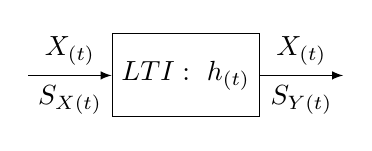
\begin{tikzpicture}[
                        node distance=2cm,
                        >=latex
                    ]
                    % Blocks
                    \node [coordinate] (input) {};
                    \node [rectangle, draw,minimum height=3em, minimum width=3em,right of=input] (filter) {$LTI:\ h_{(t)}$};
                    \node [coordinate, right of=filter] (output) {$s_{(t)}$};
                
                    % Connections
                    \draw [->] (input) --node[above]{$X_{(t)}$} node[below]{$S_{X(t)}$} (filter);
                    \draw [->] (filter) --node[above]{$X_{(t)}$} node[below]{$S_{Y(t)}$} (output);
                \end{tikzpicture}    
            \end{figure}            
            \begin{align}
                S_{Y(f)} &= TCF[R_X] =TCF[ R_{X(\tau)}\otimes h_{(\tau)} \otimes h_{(-\tau)}] \overset{\ref{Conv. Distributiva}}{=}  S_{X(f)}H_{(f)} H_{(-f)}    \nonumber \\
                         &\overset{\ref{Simmetria Hermitiana}}{=} S_{X(f)}H_{(f)} H^\ast_{(f)} =  S_{X(f)}|H_{(f)}|^2\nonumber
            \end{align}
            trovo che la densitá spettrale di potenza di $Y_{(t)}$ é la densitá spettrale di potenza di $X_{(t)}$ per il modulo quadro della
            risposta del filtro e la sua misura é in watt per hertz ($W/Hz$).
    \subsection{Processo Gaussiano}
        Un processo $Y_{(t)}$ é detto processo Gaussiano se la variabile aleatoria $Y$ é una variabile aleatoria a distribuzione Gaussiana:
        \[
            f_{Y(y)} = \frac{1}{\sqrt{2\pi}\sigma}e^{\left(\displaystyle-\frac{(y-\mu)^2}{2\sigma^2}\right)}    
        \] 
        \paragraph{Propietá:}
        \begin{itemize}
            \item {
                Il processo stocastico creato da un fenomeno fisico solitamente é possibile ricondurlo a un modella Gaussiano.
            }
            \item {
                L'uso di un modello Gaussiano per un fenomeno fisico é spesso confermato dagli esperimenti.
            }
            \item {
                Il teorema del limite centrale (\ref{Teorema del Limite Centrale - Central Limit Theorem}) fornisce una giustificazione matematica per la 
                distribuzione Gaussiana.
            }
        \end{itemize}
        \subsubsection{Rumore Bianco}
            É una sorgente di rumore idealizzata in modo tale da rendere lo spettro di densitá di potenza costante ($\frac{N_0}{2}$), cioé indipendente
            dalla frequenza a cui operiamo. L'aggettivo "Bianco" deriva dall'ottica: un segnale di luce bianca contine in ugual maniera tutte le frequenze
             all'interno dello spettro visivo. Ne possiamo dare una definizione approssimativa:
             \begin{center}
                Il rumore bianco, identificato da $W_{(t)}$ é un processo stazionario con densitá di potenza spettrale $S_{W(f)}$ con valore
                costante in tutto l'intervallo delle frequenze:
                \[
                    S_{WW(f)} = \frac{N_0}{2}\ \forall f  
                \]
             \end{center}
             \begin{figure}[H]
                \centering
                \subfloat[Densitá di potenza spettrale]{
                    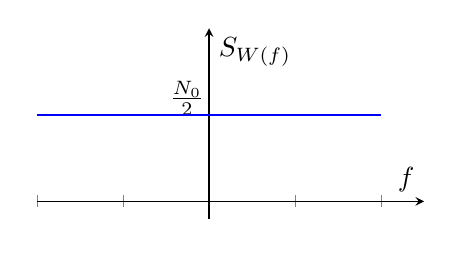
\begin{tikzpicture}
                        \begin{axis}[
                            xlabel=$f$,
                            ylabel=$S_{W(f)}$,
                            xmin=-4,
                            xmax=5,
                            ymin=-0.2,
                            ymax=2,
                            ytick = {1},
                            xtick={},
                            xticklabels={},
                            yticklabel style = {yshift=6pt,xshift=4pt}, 
                            yticklabels = {$\frac{N_0}{2}$},
                            axis lines=middle,
                            domain=-4:4,
                            samples=100,
                            width=6.5cm,
                            height=4cm
                        ]
                        \addplot [const plot, blue, thick] coordinates{(-4,1)(4,1)};
                        \end{axis}
                    \end{tikzpicture}
                }
                \hfill
                \subfloat[Autocorrelazione]{
                    \begin{tikzpicture}
                        \begin{axis}[
                            xlabel=$\tau$,
                            ylabel=$R_{X(\tau)}$,
                            xmin=-4,
                            xmax=5,
                            ymin=-0.2,
                            ymax=2,
                            ytick = {1},
                            xtick={},
                            xticklabels={},
                            yticklabel style = {yshift=5pt,xshift=4pt}, 
                            yticklabels = {$\frac{N_0}{2}\delta_{(\tau)}$},
                            axis lines=middle,
                            domain=-5:5,
                            samples=100,
                            width=6.5cm,
                            height=4cm
                        ]
                        \addplot+ [blue, thick,mark = triangle] coordinates{(0,0)(0,1)};
                        \end{axis}
                    \end{tikzpicture}
                }
            \end{figure}
            \paragraph{Propietá:}
            \begin{itemize}
                \item {Dato che $R_{W(\tau)}=0\ \forall \tau\neq 0$ ne segue che due differenti campionamenti del rumore bianco sono completamente
                incorrelati tra loro}
                \item {
                    Se il rumore bianco é Gaussiano allore due campioni sono statisticamente indipendenti.
                }
                \item {
                    Finché la banda di un processo del rumore in ingresso al sistema é ampiamente maggiore della banda del sistema stesso, allora possiamo modellare
                    il rumore come un processo a rumore bianco.
                }
            \end{itemize}
        \subsubsection{Filtro passa basso ideale per rumore bianco}
            Supponiamo di avere un ricevitore:
            \begin{figure}[H]
                \centering
                    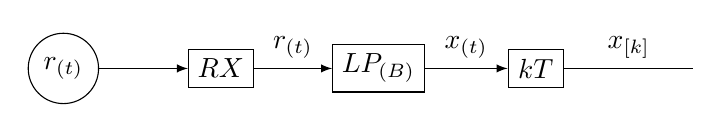
\begin{tikzpicture}[
                            node distance=2cm,
                            >=latex
                        ]
                        % Blocks
                        \node [circle,draw] (RXant) {$r_{(t)}$};
                        \node [rectangle, draw,minimum height=1em, minimum width=2em,right of=RXant] (RX) {$RX$};
                        \node [rectangle, draw,minimum height=1em, minimum width=2em,right of=RX] (DC) {$LP_{(B)}$};
                        \node [rectangle, draw,minimum height=1em, minimum width=2em,right of=DC] (DS) {$kT$};
                        \node [coordinate,right of = DS] (output) {};
                    
                        % Connections
                        \draw [->] (RXant) --node[above]{} (RX);
                        \draw [->] (RX) --node[above]{$r_{(t)}$} (DC);
                        \draw [->] (DC) --node[above]{$x_{(t)}$} (DS);
                        \draw [-] (DS) --node[above]{$x_{[k]}$} (output);
                    \end{tikzpicture}    
            \end{figure}
            e un rumore additivo:
            \begin{figure}[H]
                \centering
                    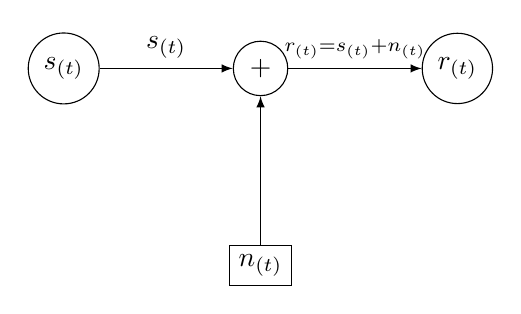
\begin{tikzpicture}[
                            node distance=2.5cm,
                            >=latex
                        ]
                        % Blocks
                        \node [circle,draw] (TXant) {$s_{(t)}$};
                        \node [circle, draw,right of=TXant] (sum) {$+$};
                        \node [rectangle, draw,below of = sum,minimum height=1em, minimum width=2em] (error) {$n_{(t)}$};
                        \node [circle,draw,right of=sum] (RXant) {$r_{(t)}$};
                    
                        % Connections
                        \draw [->] (TXant) --node[above]{$s_{(t)}$} (sum);
                        \draw [->] (sum) --node[above]{$\scriptstyle r_{(t)} = s_{(t)}+ n_{(t)}$} (RXant);
                        \draw [->] (error) -- (sum);
                    \end{tikzpicture}    
            \end{figure}
            inviamo un segnale $s_{(t)}$ con banda $B$:
            \begin{figure}[H]
                \centering
                \subfloat[Trasmettitore]{
                    \begin{tikzpicture}
                        \begin{axis}[
                            xlabel=$f$,
                            ylabel=$S_{W(f)}$,
                            xmin=-5,
                            xmax=5,
                            ymin=-0.2,
                            ymax=1,
                            ytick = {1},
                            xtick={-2,2},
                            xticklabels={$-B$,$B$},
                            yticklabel style = {yshift=6pt,xshift=4pt}, 
                            yticklabels = {$\frac{N_0}{2}$},
                            axis lines=middle,
                            domain=-5:5,
                            samples=800,
                            width=6.5cm,
                            height=4cm
                        ]
                        \addplot [const plot, blue, thick, domain = -2:2] {gauss(0,0.8)-0.01};
                        \end{axis}
                    \end{tikzpicture}
                }
                \hfill
                \subfloat[Ricevitore: ${\color{blue}s_{(t)}}+ {\color{purple}n_{(t)}}$]{
                    \begin{tikzpicture}
                        \begin{axis}[
                            xlabel=$\tau$,
                            ylabel=$R_{X(\tau)}$,
                            xmin=-5,
                            xmax=5,
                            ymin=-0.2,
                            ymax=1,
                            ytick = {1},
                            xtick={-2,2},
                            xticklabels={$-B$,$B$},
                            yticklabel style = {yshift=5pt,xshift=4pt}, 
                            yticklabels = {$\frac{N_0}{2}\delta_{(\tau)}$},
                            axis lines=middle,
                            domain=-5:5,
                            samples=800,
                            width=6.5cm,
                            height=4cm
                        ]
                        \addplot [const plot, blue, thick, domain = -2:2] {gauss(0,0.8)-0.01};
                        \addplot [const plot, purple, thick] coordinates{(-5,0.2)(5,0.2)};
                    \end{axis}
                    \end{tikzpicture}
                }
                \
            \end{figure}
            il ricevitore si occupa adesso del filtraggio con un filtro passa basso di banda $B$ ($LP_{(B)}$), ritrovando il 
            segnale originale ma con il rumore additivo:
            \begin{figure}[H]
                \centering
                \begin{tikzpicture}
                    \begin{axis}[
                        xlabel=$\tau$,
                        ylabel=$R_{X(\tau)}$,
                        xmin=-5,
                        xmax=5,
                        ymin=-0.2,
                        ymax=1,
                        ytick = {0.6},
                        xtick={-2,2},
                        xticklabels={$-B$,$B$},
                        yticklabel style = {yshift=5pt,xshift=4pt}, 
                        yticklabels = {$1$},
                        axis lines=middle,
                        domain=-5:5,
                        samples=800,
                        width=8cm,
                        height=5cm
                    ]
                    \addplot [const plot, blue, thick, domain = -2:2] {gauss(0,0.8)-0.01};
                    \addplot [const plot, purple, thick] coordinates{(-5,0.2)(5,0.2)};
                    \addplot [const plot, orange, thick] coordinates{(-5,0)(-2,0)(-2,0.6)(2,0.6)(2,0)(5,0)};
                \end{axis}
                \end{tikzpicture}
                \caption{${\color{blue}s_{(t)}},{\color{purple}n_{(t)}},{\color{orange}LP-filter}$}
            \end{figure}
            in uscita dal filtro ho $x_{(t)} = s_{(t)} + n_{(t)} \otimes h_{(t)}$ con la densitá spettrale del rumore:
            \[
                S_{W(f)} = S_{n(f)} |H_{(f)}|^2 = S_{n(f)} 
            \]
            Per ricostruire il segnale devo campionare con una $f_s = \frac{1}{T_s} = 2B$ ($kT$):
            \[
                x_{[k]} = x_{(t=kT)} = s_{[k]}+w_{[k]}    
            \]
            Cosa succede al rumore?
            Nel dominio della frequenza lo spettro di rumore filtrato,$w_{[k]}$, é  una somma di delta di dirac ho quindi $S_{w(f)} = rect\left(\frac{f}{2B}\right)$
            trasformadola nel dominio del tempo, cioé calcolando la sua autocorrelazione per $ATCF[S_{w(f)}] = R_{w(\tau)}$ ottengo $R_{w(\tau)} = 2B\tau sinc(2B\tau)$,
            campionandola rispetto alla banda del filtro $B$ in $\frac{k}{2B}$ la $sinc$ é sempre $0$ rendendo le variabili del rumore Gaussiano statisticamente 
            indipendenti a valore medio nullo e varianza $N_0B$. 
            \[
                \eval*{R_{w(\tau)}}_{\tau=kT} =\eval*{\mathbb{E}[w_{(t)}w_{(t-\tau)}]}_{\tau=kT} \overset{T=\frac{1}{2B}}{=} 0  
            \]
            \begin{figure}[H]
                \centering
                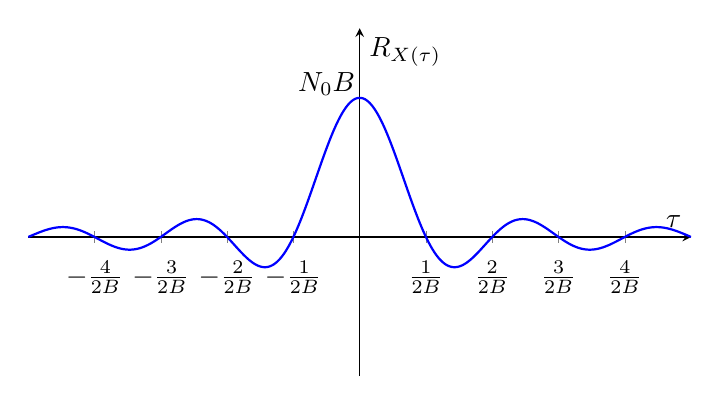
\begin{tikzpicture}
                    \begin{axis}[
                        xlabel=$\tau$,
                        ylabel=$R_{X(\tau)}$,
                        xmin=-5,
                        xmax=5,
                        ymin=-1,
                        ymax=1.5,
                        ytick={1},
                        yticklabels = {$N_0B$},
                        yticklabel style = {yshift=5pt,xshift=4pt}, 
                        xtick={-4,-3,-2,-1,1,2,3,4},
                        xticklabels={$-\frac{4}{2B}$,$-\frac{3}{2B}$,$-\frac{2}{2B}$,$-\frac{1}{2B}$,$\frac{1}{2B}$,$\frac{2}{2B}$,$\frac{3}{2B}$,$\frac{4}{2B}$},
                        xticklabel style = {yshift=-3pt}, 
                        axis lines=middle,
                        domain=-5:5,
                        samples=800,
                        width=10cm,
                        height=6cm
                    ]
                    \addplot [blue, thick, samples = 800] {sin(deg(x*pi))/(x*pi)};
                \end{axis}
                \end{tikzpicture}
            \end{figure}
            per questo il modello $Y = S + n \sim \mathcal{N} (0,\sigma^2)$ é giusto per approssimare il rumore. Calcoliamone il valor medio e varianza:
            \begin{gather}
                w_{(t)} \sim \mathcal{N}(0,\sigma^2_w)  \nonumber \\
                \sigma^2_w = \mathbb{E}[X^2]-\mu_w = \mathbb{E}[X^2] = R_{w(0)} = N_0B\nonumber
            \end{gather}
            Ne segue che piú la banda é elevata piú rumore entra nel sistema.            






